\section{From Extended Circle Patterns to polyhedra}

In this section, we describe how to obtain a
decomposition of a torihedron
into hyperbolic ideal pyramids
from a non-singular extended circle pattern.

\begin{lemma}
\label{l:circpattern_polyhedra}
Suppose we have the graph of a torihedron.
Given a non-singular extended circle pattern $c \in \CCC$ on the graph,
such that all $\vphi_{\vec{e}} \in (0,\pi)$,
there exists a decomposition of the torihedron
into base-angled ideal pyramids (TODO make sure it's been defined) such that
	\begin{itemize}
		\item each interior edge of the torihedron has dihedral angles sum to $2\pi$;
		\item each boundary edge $e$ of the torihedron has dihedral angles sum to
			$\pi - \theta_e$.
	\end{itemize}
\end{lemma}

\begin{proof}
For each directed edge $\vec{e} \in \vec{E}$,
construct the isosceles triangle $T_{\vec{e}}$
with equal sides of length $r_{f_{\vec{e}}}$ and
angle $2\tilde{\vphi}_{\vec{e}}$ subtended between them,
where $\tilde{\vphi}_{\vec{e}} = \vphi_{\vec{e}}$
if $\vphi_{\vec{e}}$ if it is acute,
and = $\pi - \vphi_{\vec{e}}$ otherwise.

\begin{figure}
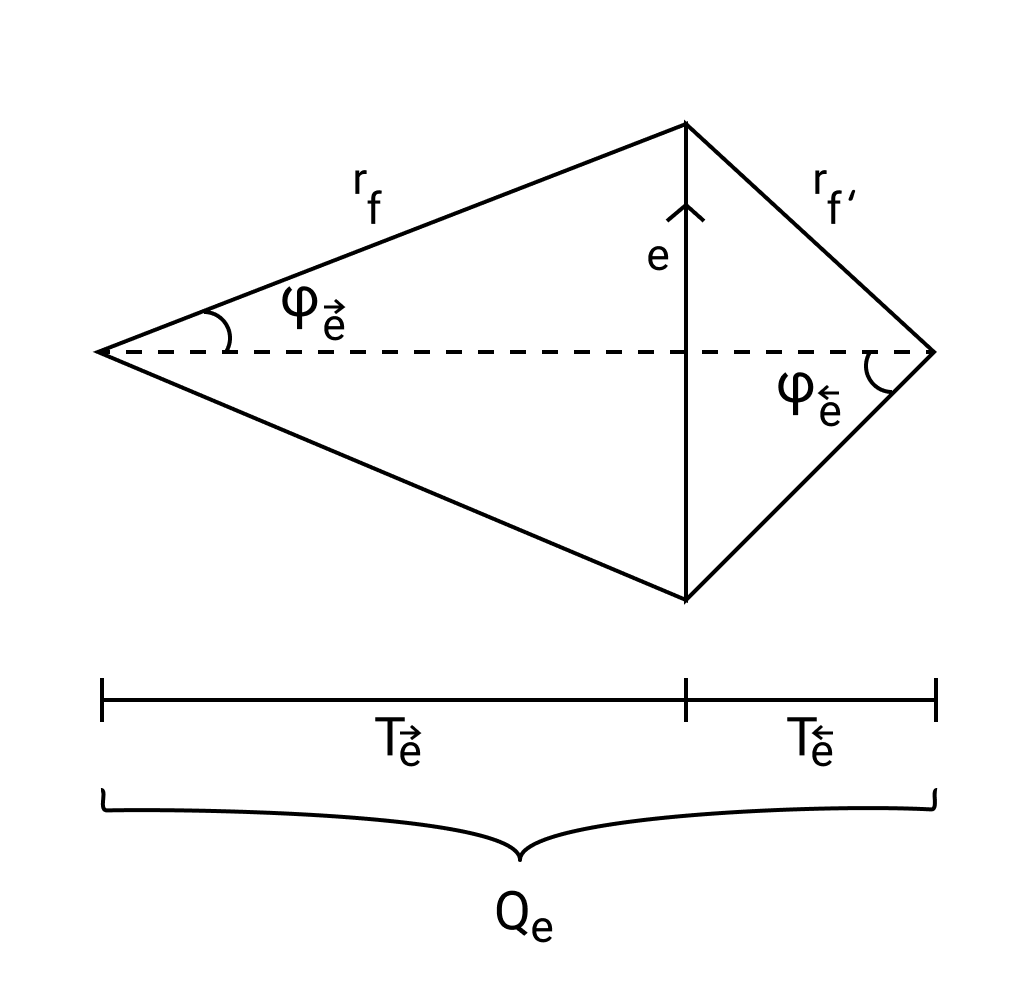
\includegraphics[width=8cm]{more_pictures/kite.png}
\end{figure}
\begin{figure}
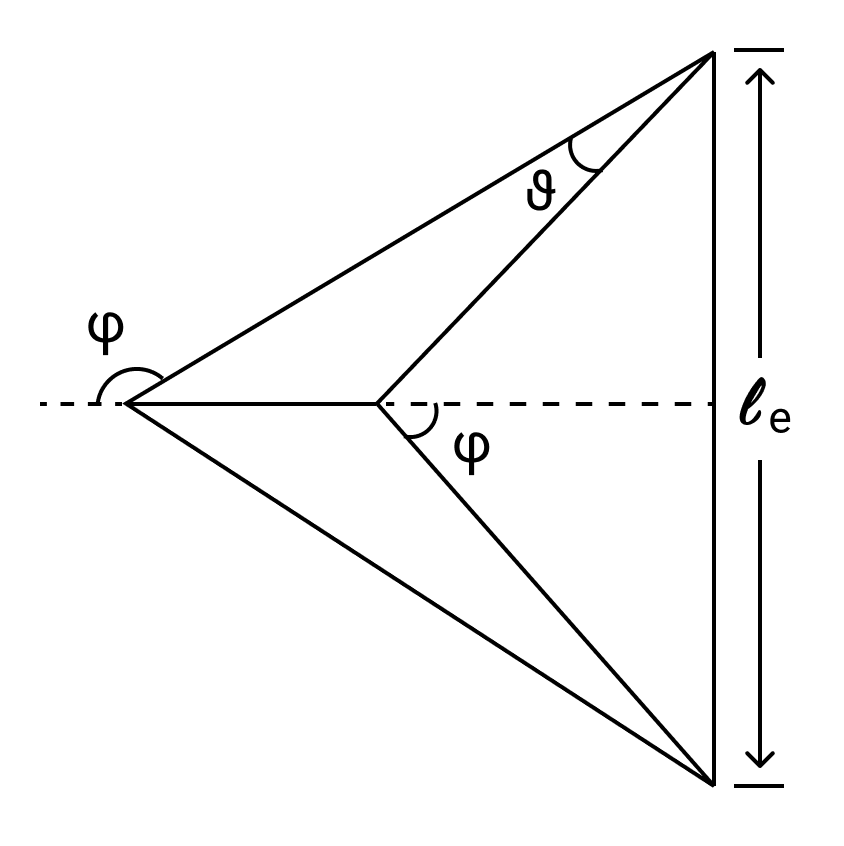
\includegraphics[width=5cm]{more_pictures/positive_angle.png}
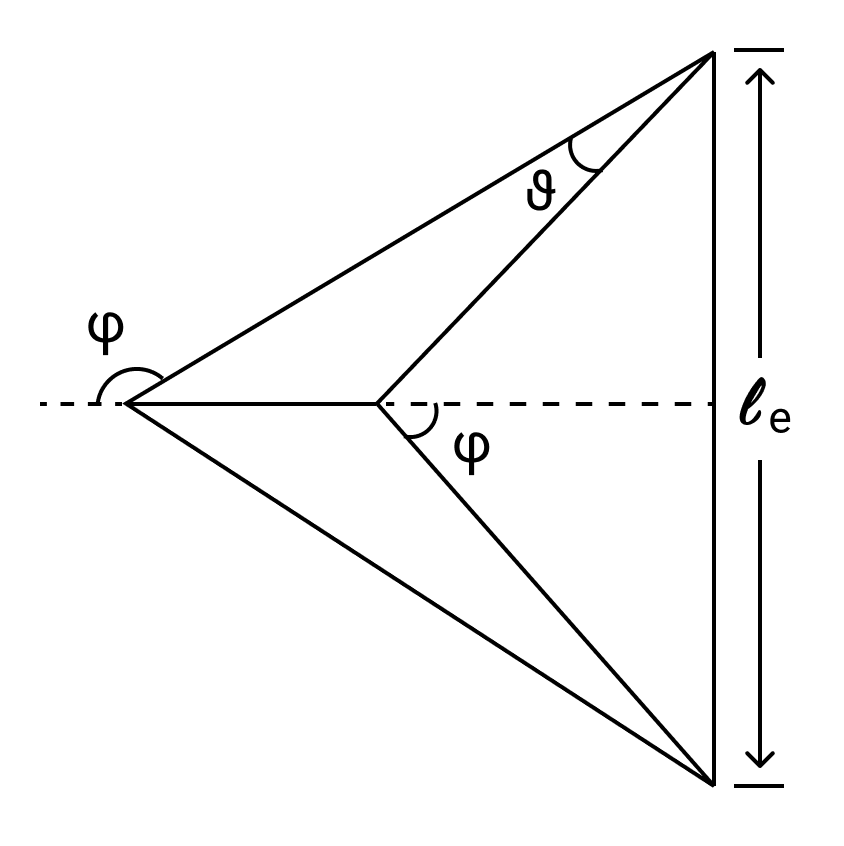
\includegraphics[width=5cm]{more_pictures/negative_angle.png}
\end{figure}


Let $f \in F$ be a face.
We construct a Euclidean polygon $\Pol_f$ as follows.
If $\vphi_{\vec{e}} \leq \pi/2$ for all $\vec{e} \in \del f$,
i.e. if $f$ is convex, then 
the $T_{\vec{e}}$ for $\vec{e}\in \del f$
fit together into $\Pol_f$.
If not, suppose $\vphi_{\vec{e}} > \pi/2$
for $\vec{e} = \vec{e_1}$, 
and $\leq \pi/2$ for $\vec{e} = \vec{e_2},\ldots \vec{e_k} \in \del f$.
Then put $T_{\vec{e_2}},\ldots,T_{\vec{e_k}}$ together as above,
creating a $(k+1)$-gon,
then subtract $T_{\vec{e_1}}$ from it to form $\Pol_f$.

Thus, to each face, we associate the Euclidean polygon $\Pol_f$.
If $v$ is the vertex of $\Pol_f$ between $e_i$ and $e_{i+1}$,
then the angle at $v$ is
$\pi - \vphi_{\vec{e_i}} - \vphi_{\vec{e_{i+1}}}$.
Then the non-vertex-singularity of $c$ guarantees that
the sum of angles at $v$ of $\Pol_f$, for faces $f$ containing $v$,
is $2\pi$.
%; in other words, $\Pol_f$ glue along edges


View the Euclidean plane as the boundary of the upper-half space.
Then $\Pol_f$ supports an ideal hyperbolic pyramid $P_f$.

Clearly, these $P_f$'s, as abstract ideal tetrahedra,
glue together into the torihedron (TODO rephrase).
%The hyperbolic structure on $P_f$
%in particular provide dihedral angles to each edge of $P_f$
%which clearly satisfies the conditions of making $P_f$
%a base-angled ideal pyramid.
We need to check that the angles around each edge of
the torihedron have the appropriate angles.


Consider an interior edge $e$ of the pyramidal decomposition
of the torihedron.
It corresponds to a vertex $v$ of the graph.
Note that the dihedral angle of the vertical edge
at $v$ of $P_f$ is simply the angle at $v$ of $\Pol_f$;
these sum to $2\pi$ over $f \ni v$.


For a boundary edge $e$, the dihedral angles at $e$ of the $P_f$'s
containing it are $\vphi_{\vec{e}}$ and $\vphi_{\cev{e}}$,
which sum to $\theta_e$ by definition.

\end{proof}
